\section{Introduction}

The subject of nuclear physics investigations is correlated many-body system of strongly interacting fermions. 
Although, the objects of such investigations are mostly just two-component systems, consisted of neutrons and protons (nucleons), the limits of such investigations are very far by the present moment.
However, more than three thousand proton-neutron configurations, isotopes, have been already discovered.
And one cannot speak about the exact number of them, because it is continuously growing. 
The theoretical estimation predict that from 2000 to 3000 other nuclear systems can be synthesized.  
All the nuclei can be classified by the number of nucleons (A), comprising the proton (Z) and neutron number (Z). 
These variables are the members of the famous Bethe–Weizs{\"a}cker mass formula, which is used to approximate the mass of the nuclei \textcolor{red}{[???]}.
\begin{equation}
	E_{T} = a_{1}A - a_{2}A^{2/3} - a_{3}\frac{Z(Z-1)}{A^{1/3}} - a_{4}\frac{(N-Z)^2}{A} + \delta(N,Z).
	\label{eq:BetheWeizs}
\end{equation}
This formula represents the liquid drop model proposed by George Gamow, in which the atomic nucleus is regarded as the spherical drop of non-compressible charged nuclear liquid.
This model is based on the well-known symmetry of the strong interactions for neutrons and protons and also involved the surface effects, short-range character of the force, electromagnetic repulsive contribution, assymetry energy and proton-neutron pairing.
And as it turns out, that the simple reasoning of the charged liquid drop model allow to predict the mass of most stable nuclei with fairly good accuracy.
Based on the ideas, one can suggest, that nuclei have a spherical shape and due to the pairing phenomenon, have relatively similar number of neutrons and protons.
The nuclear chart in Fig.\ \ref{fig:nuclear_chart}, shows that especially for light nuclei, located in the valley of stability and colored in black, the number of neutrons is approximately equal to the number of protons.
In this work we determine isotopes with A<20 as light nuclei.
For heavy systems, due to the Coulomb repulsion and short range of the nuclear forces, the ratio of mass over charge is increasing and reaches the value of 1.6 in a region of A>250. 

%-------------------------------------------------------------------------------
\begin{figure}[t]
	\begin{center}
		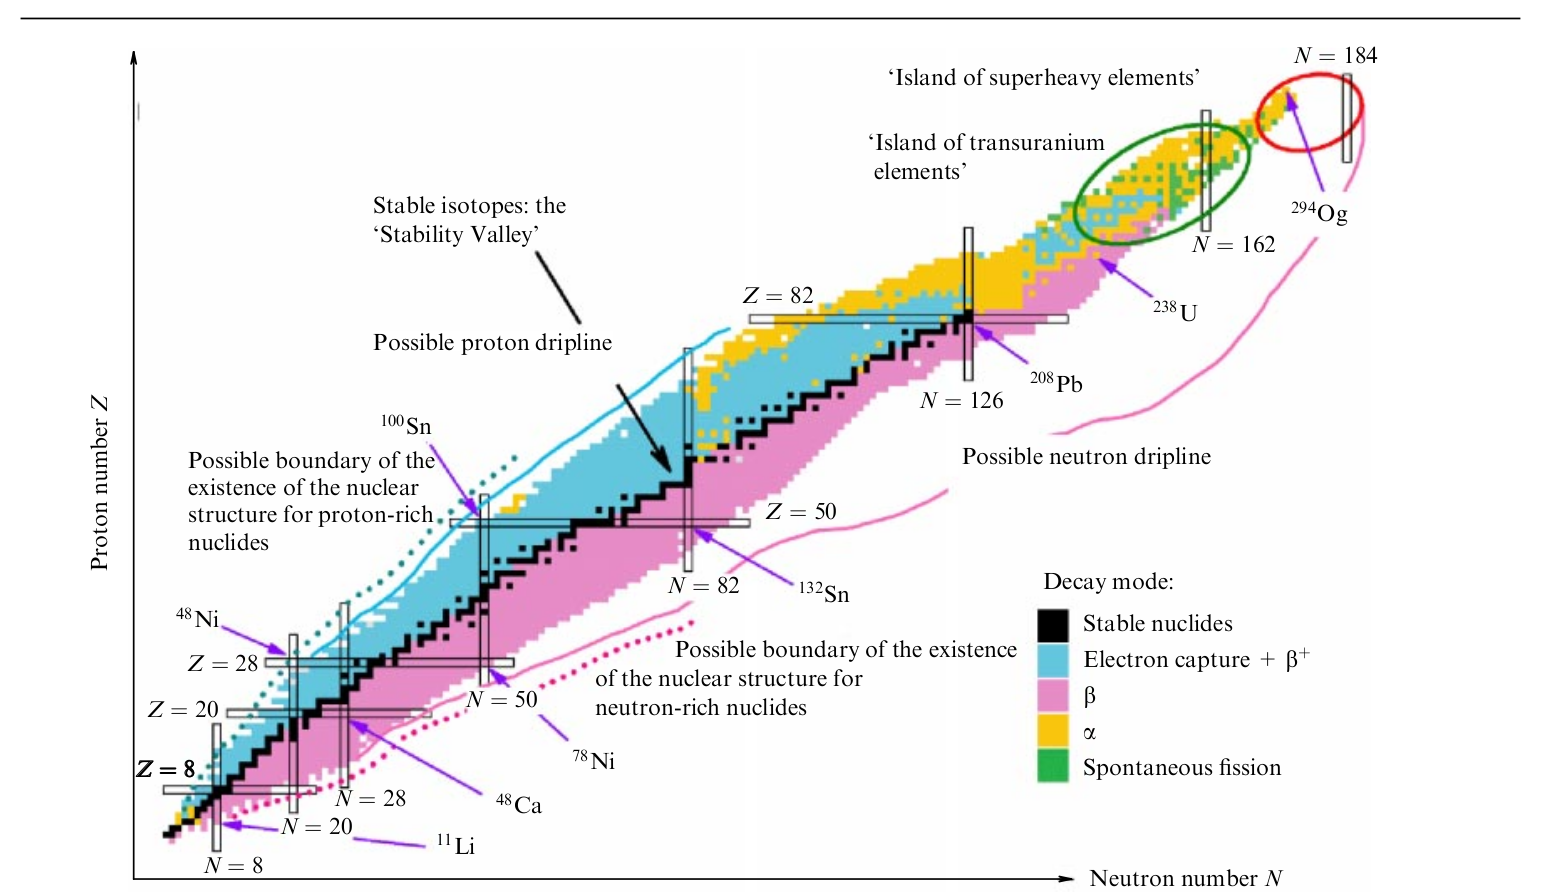
\includegraphics[width=1\textwidth]{figures/map.png}
	\end{center}
	%
	\caption{Illustration of global structures in the nuclear chart. 
		The chart of nuclides is an analog of the periodic table for nuclear physics. 
		In atomic physics, the main regularities are connected with the order in which the electron shells in atoms are filled. 
		In nuclear physics, similar dependences are connected with the sequence in which the nuclear shells are filled for two types of particles, protons and neutrons. 
		Vertical and horizontal bands indicate the `magic' numbers corresponding to the number of protons Z and the number of neutrons N. 
		Some 'special' nuclides are indicated by arrows: $^{11}$Li is a nuclide with one of the most developed 'Borromean' two-neutron haloes, double-magic nuclides in long isobaric chains; $^{294}$Og is the heaviest nuclide known today.}
	%
	\label{fig:nuclear_chart}
\end{figure}
%-------------------------------------------------------------------------------

It is known that there are 243 stable nuclei, but in nature one can find about 339 \cite{Grigorenko:2016}. 
That means, that some of them are unstable with respect to $\alpha-$, $\beta-$ or $\gamma-$decay and fission (for heavy elements), but they are still bound and live long enough to come down to us from the early universe, or are decay products of heavier nuclear systems. 
Bound nuclear systems are defined by mean of single or multiple nucleon separation energy.
As further the isotope is located on from the line of stability Fig.\ \ref{fig:nuclear_chart}, the less is the separation energy.
At some point the system becomes so unstable, so it becomes energetically favorable to emit one or several nucleons.
The borders between bound and unbound nuclear systems are called driplines.
One can also notice that there are many driplines, related to different decay processes.
Here one should draw the line between the concept of radioactivity and decay. 
Radioactivity is the phenomenon, related to the atomic systems, which implies the atomic orbitals formation.
That is why, the term radioactivity can be used only for long-lived systems, while the decay concept applies to the strictly nucleon systems.
Beyond the driplines nuclear systems can exist as so-called resonances. 
All resonances, together with exotic nuclei, located in the vicinity of the driplines, are called exotic nuclear systems.
Usually, as more exotic the system is, the less its lifetime, which makes studies of exotic states challenging. 
That is why the location of the driplines was experimentally obtained only for the light nuclei \cite{GrigorenkoUFN:2019}.
And moreover, so far there is no answer to a fundamental question: how far beyond the dripline can the resonances be located? 
And moreover, it remains an open important fundamental question as to whether the border between unbound nuclear systems and continuous spectra is existed, and where is it located.

Aside from the experimental issues of studies of short-lived exotic nuclear systems, there are no universal theoretical models, describing the nuclear matter under such extreme conditions.
The reason for this is that exotic systems differ from the nuclei located in a line of stability not only in Z/A ration but also in unique phenomena existence.
Halo and skin effects, different magic shell numbers, new types of excitation and radioactivity make most of the nuclear structure models inapplicable for description of such unstable systems.

\begin{itemize}
	\item 
	One can suggest that in exotic nuclear systems, those valence nucleons, occupied the highest shells, can tunell to the classically forbidden regions. 
	The manifestations of such phenomenom are the different spatial distribution of the valence nucleons, compared to others. 
	That is why, such transformed systems have larger corresponded radii than their stable isotopes.
	One can imagine such system as cluster-core, surrounded by the valence nucleons with smaller separation energy.
	It leads not only to abnormal large nuclear radius, see Fig.\,\ref{fig:halo_skin_density}, but other anomalies, such as reaction cross section increasing, very narrow momentum distribution of the valence nucleons, etc.
	For the fist time, the term "halo" was used in the work Ref.\ \cite{Hansen:1987}, but by the present day, it is well known, that such exotic feature was observed in many neutron-rich ($^{6}$He, $^{11}$Li,$^{17}$B, $^{19}$B, $^{22}$C) and neutron-deficient systems ($^{8}$B, $^{13}$N, $^{17}$Ne, $^{26}$P, $^{27}$S) \textcolor{red}{[some cite to the HALO summary report]}.
	In the systems with neutron excess, so-called "neutron skin" phenomenon can be also observed.
	Such systems are characterized by the extension of size, but not the form, illustrated in Fig.\,\ref{fig:halo_skin_density}. 
	$^{8}$He and $^{14}$Be are well known examples of the isotopes with neutron skin.
	
	%-------------------------------------------------------------------------------
	\begin{figure}[t]
		\begin{center}
			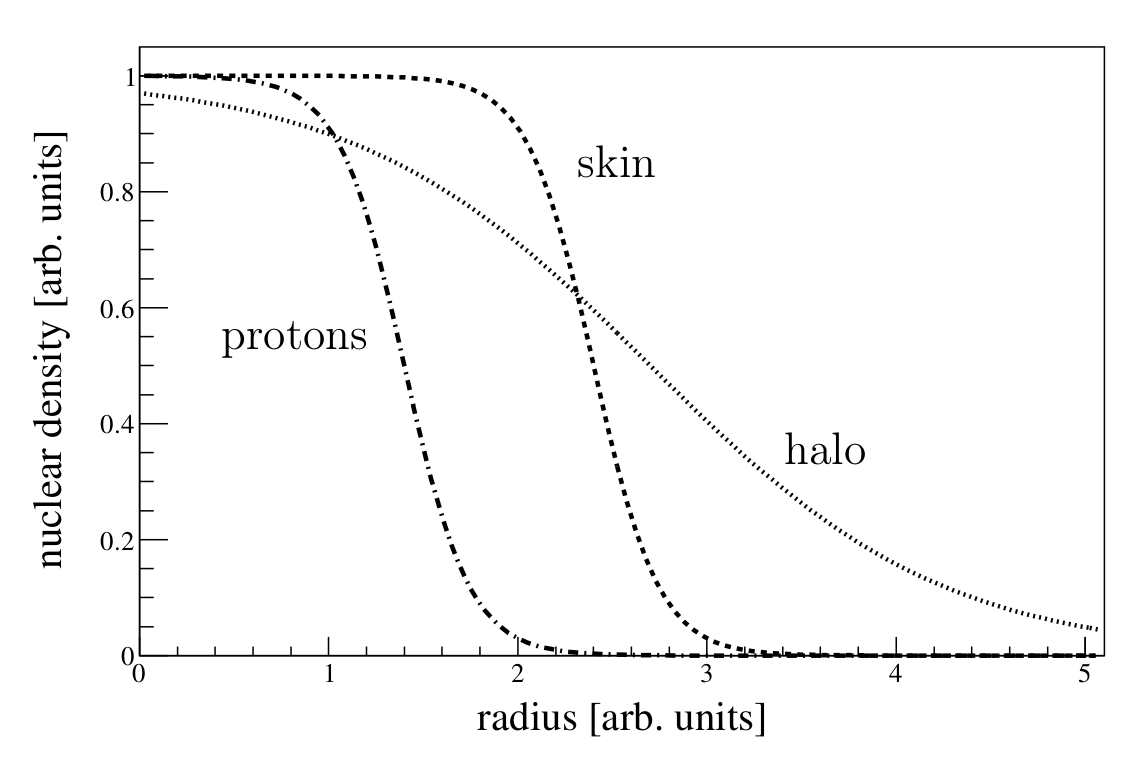
\includegraphics[width=0.7\textwidth]{figures/densityDistr.png}
		\end{center}
		%
		\caption{
			Illustration of nuclear matter density for nuclear halo and skin. 
			Density of proton matter is depicted by dashed-and-dot line; nuclear skin presented by dashed
			line is characterized by larger radius than core matter; and matter distribution of
			nuclear halo depicted by dotted line is less compact and more spread in comparison
			with nuclear skin.}
		%
		\label{fig:halo_skin_density}
	\end{figure}
	%-------------------------------------------------------------------------------
	
	\item 
	The spatial transformations of nucleons lead to the new freedom degree, so-called soft excitation mode, which can be described as oscillations of the valence nucleons with respect to the core cluster. 
	
	\item 
	Some core-halo nuclear systems may represent so-called "Borromean nuclei", which were named after the Borromean rings - the mathematical object, consisted of three topologically licked curves, which cannot be separated, but not without any binary links between each other.
	Removing any part of it, one disintegrate the whole system.
	In other words, Borromean nuclei are bound only as many-body system, while all its subsystems are unbound.
	This has led to simultaneous many-body decays of some exotic nuclear systems, which can not occur sequentially, due to the separation energy conditions.
	

\end{itemize}



Studies of the light exotic nuclear systems take a particular significant role in modern physics.
The limited number of nucleons of light isotopes allows to highlight the contribution of the studied phenomena effects among other processes, which is extremely convenient for reactions of exotic system production, characterized by low cross sections.
On top of that, in the light isotopes the extreme of ratio of mass-over-charge can be reached.
These short-lived systems are usually characterized by many-body decay channels.

Investigation of such simultaneous many-body decays is the only way to get experimental information about the many-body capture processes, which can be considered as the time reversal reactions to the observed decays.
These processes may occur only in under extreme conditions of very high temperature and density, that is why investigations of exotic nuclear systems may have a significant contribution to astrophysics.
%Both fast mechanisms of nucleosynthesis (r- and rp-processes), occurred in compact objects with isotopes, located nearby both proton and neutron driplines. 
For example, investigations of the neutron-deficient systems in the vicinity of the proton dripline can be an instrument to study the nucleosynthesis of fast proton-capture, so-called rp-process, occurred on the surface of a neutron stars in a reactions of hydrogen burning \cite{GrigorenkoUFN:2019,Grigorenko:2009b,Grigorenko:2006,Grigorenko:2005a,Schatz:1998}. 
The features of this rp-process at waiting points, at which single proton capture is forbidden, can be explored using the reactions of multi-proton decays \cite{Gorres:1995}.
On the other hand, the rapid neutron-capture process, also known as the r-process, proceeds along the neutron dripline in supernova core-collapse processes, is similarly studied in reactions with neutron-rich isotopes.
Therefore, investigation of multi-nucleon emitters is a good test for developing theoretical models, which are supposed to provide the equation of state of the nuclear matter at extreme conditions. 

\subsection{Experimental techniques for exotic nuclear research}

Due to the short lifetime, exotic nuclei can not be found in nature.
And even with modern technologies, studies of such abnormal systems is a great technical challenge due to low cross sections of the reactions of interest, extremely short lifetimes of the systems of interest and overwhelming production of unwanted species in the same target.
New isotopes can be products of either compound or direct nuclear reactions.

The compound reactions are slow-collisions with so-called adiabatic conditions \cite{Zagrebaev:2019}.
In such collisions the target-projectile relative speed is incomparable to the Fermi velocity (speed of a nucleon within the nucleus), which allows to share the total energy of projectile and target among all the nucleons of the compound system.
In such \textbf{fusion reactions} the system with N-Z combination, approximately equal to the sum of the number of protons and neutrons in the initial beam and target nuclei, is produced.
Due to the increasing asymmetry of mass over charge for heavy nuclei, such reaction mechanism is commonly used in studies of neutron-deficient isotopes.
If the compound nucleus has too much energy to be stable, it decay into two or many fragments, and thus produce nuclei with big mass-charge asymmetries.

At the opposite extreme are the direct nuclear reactions, in which the projectile interacts with only few fragments of the target, involving only small number of degrees of freedom.
Different mechanisms of the direct reactions can be used in studies of exotic nuclear states. 

\begin{itemize}
	
	\item 
	\textbf{Pickup or stripping transfer reactions} are widely used mechanisms, especially for light system research, in which the beam exchanges the nucleons with a beam. 
	Stripping is transfer from the projectile to the target, and pickup from the target to the projectile.
	
	\item
	In the \textbf{knock-out reactions}, the isotopes can be produced in a single nucleon or a light cluster removal process from the projectile by a collision with the target.
	
	\item
	In order to obtain exotic nuclei, the \textbf{charge-exchange reactions} can be applied.
	In these reactions predominantly  the ground state of exotic product is populated by replacing of one or few protons (neutrons) with neutrons (protons).
	
	
\end{itemize}	
Direct reactions occur with high probability with light particles, and can be can be easily identified.
%But, probably, the main advantage of using such reaction mechanisms is the possibility 
Due to the very small amount of involved degrees of freedom, only few final states of the studied system can be populated, which makes experiments with such reactions one of the best tools to selectively study the properties of specific states.

Eventually, over time, the capabilities of the described methods with stable beams were exhausted.
The idea of using radioactive ion beams (RIB) was a breakthrough approach in search of new isotopes, which allowed to significantly extend the frontiers of known isotopes. 
Despite to the continuous technological progress, the main problem of usage RIB is their short lifetime (less than 1 second), which requires to develop new specific methods of the beam transport system.

%The nuclei of interest, forming the desired secondary RIB, are extracted and separated by one of the separation methods.

In general, there are two main separation techniques to make the good quality RIB: the isotope separation on-line (ISOL) and the in-flight separation methods.
In both methods the RIB is produced through different reaction mechanisms of interaction of the stable primary beam with a thick production target, made of heavy elements.
Both methods transport the isotopes of interest, forming the secondary beam, away from production target, where a large background from nuclear reactions is present, to a experimental setup.
Apart from creating low-background conditions nearby the physical target of the experiment, the ion optical secondary beam transport system can serve as separator and post-accelerator.

Historically, the first developed approach of the RIB production was ISOL method. 
The production target applied in this method is thick enough to stop all the beam particles inside.
Nuclear collisions inside the target volume cause the fragmentation processes of the heavy nuclei of the production target, which produce multiple isotopes.
The cooled particles of interest are extracted and undegro ionization, forming the secondary RIB of low energies (less than 500 keV).
The modern ISOL-facilities provide the extraction time of less than 0.1 second.
Depending on the lifetime of the corresponded particles, the secondary beam can pass through several separation, acceleration and focus stages implemented by standart ion optical facilities of the fragment separator.	
The described principles employed for production of the RIB consisted of only long lived isotopes, but allow one to reach very high intensity and purity of the secondary beam.

In-flight method is the most common for production of short lived (but with $T_{1/2}>50\,$ns) RIBs. 
Another its advantage is the possibility to obtain a very rich RIB cocktail, because the set of the used reactions, occurred in the production target, is much wider than in the ISOL technique. 
The energies of the primary beam can vary from 30\,AMeV (per nucleon) to 1\,AGeV.
The in-flight method required to use relatively thin target, so all the fragments can leave the production target volume at forward angles to the primary beam direction. 
In order to reach the high qualities of the RIB, within the very strict time limits, the secondary beam transport system requires more careful diagnostics of all beam properties, implemented by the fragment separator facilities.
The beam quality plays a key role in the experimental resolution of the studied system.
Since the lifetime of the desired exotic system is extremely small and can not be measured directly, the properties of interest are usually reconstructed from the reaction products by one of widely used methods.
\begin{itemize}
	\item 
	The missing-mass (MM) method is so named because for its realization the detection of the studied system itself is not required, but calculated as a missing component of the four-momentum conservation law.
	All other particles, involved in the studied reaction are measured or known in advance (in a case of a target). 
	This method is easy to use and has high experimental resolution, which greatly increases statistics.

	\item 
	Another reconstruction algorithm would imply registration of all decay products of the studied system and called invariant-mass (IM) method.
	Although it is technically complex to realize but more accurate, which means that it can provide much better energy and angular resolution.
	
	\item 
	The fresh combined-mass method is combination of the MM method with the registration of some decay products of the exotic isotope.
	Although, it is very situational, in some cases, such technique can be the best choice and provide the highest accuracy. 
	 
	 
\end{itemize}	


This thesis is devoted to studies of light neutron-rich exotic nuclear systems, produced in direct transfer reactions at ACCULINNA-2 fragment separator.
The heavy neutron excess isotopes of the first four chemical elements allow to synthesize the system with the biggest ratio of mass over charge, approaching the neutron matter study.
This huge unique asymmetry allows different exotic features described above to be observed by the developed experimental techniques.

Outline of the Thesis
\textcolor{red}{copy from chudoba thesis}

One should mention somehow that we use h==c==1 unit system









